\chapter{Implementace frontendu}
Frontend byl vyvíjen jako single-page aplication pomocí javasriptu a reactu.
Navržen tak aby byl jednuduše ovladatelný přehledný a především velmi rychlý.

\section{Server}
Celá aplikace frontendu je uložena na serveru, včetně zdrojových kódů.
Uživatel si ale stahuje pouze zkompilovanou aplikaci a případné externí zdroje.
\subsection{Kompilace}
Ačkoliv je javascript scriptovací jazyk a kompilaci provádí až za běhu, tak je možné
jej zkompilovat předem. Při této kompilaci knihvny \textbf{webpack} a
\textbf{babel} provedou několik zásadních kroků, z nichž nejdůležitějsími jsou
projití kódu a jeho převedení na ECMAScript 5 (kvůli zpětné kompabilitě), přetřízení a sloučení
knihoven do jednoho zdrojového souboru (javascript se k uživateli dostane při prvním dotazu na server) a
minifikace výsldného souboru, jež dokáže inteligentně projít kód a optimalizovat jeho textovou délku,
čím výrazně sníží čas potřebný k načtení stránky. 
\subsection{NPM}
Celá aplikace má strukturu balíčku NPM (node package manager), tudíž ji lze snadno
spustit kdekoliv, kde je nainstalovaný nodejs a knihovna npm.
Zároveň udržuje pomocí souboru \textbf{package.json} přehled o potřebných knihovnách (dependencies) a
obsahuje též různé spouštěcí scripty, např. script pro buil produkční erze aplikace.

\section{Knihovny}
Aplikace se skládá z více než tisíce knihoven a modulů, tudíž se podíváme
pouze na ty nejvetší a nejdůležitější z nich.

\subsection{React}
Tato JavaScriptová knihovna je vyvinuta společností Facebook a slouží pro tvorbu uživatelského rozhraní.\\
Jejím základem je vykreslování pomocí tkz. single-page a je vhodná zejména pro aplikace, kde se často mění data.
Využívá pozměněné JavaScriptové syntaxe známe jako JSX (JavaScript XML), která umožňuje
pracovat s HTML tagy uvnitř JavaScriptového kódu, bez nutnosti práce DOM objektem.\\
Výhodou single-page aplikace je pak i optimalizovaná práce s DOM objektem, který je bottleneck
(úzkým hrdlem) při nesprávném použití (nebo lépe řečeno, při kterémkoliv použití, které něco s DOM objektem dělá).

\subsection{Material-ui}
Společnost Google (aktuálně Alphabet Inc.) se v roce 2014 rozhodla sjednotit svou grafickou podobu a
vyvynula designový jazyk, jež se stal příručkou jak vytvářet uživatelsky přívětivé aplikace (nejen na webu, ale třeba
i v aplikaci mobilním telefonu nebo tabletu). Základem tohoto stylu je realistická práce se světlem
a uživatelskou interakcí. Vše odlehčené a intuitivní. Součástí tohoto grafického jazyka jsou i
lehce čitelné fonty (Roboto), pochopitelné ikonky a systém barev a jejich kombinací.

\subsection{i18n}
Jelikož je projekt mířen i na nečeské uživatele, vyskytla se potřeba rozhranní překládat.
Jednoduchým přístupem by bylo zkompilovat několik aplikací každou pro jiný jazyk, tudíž
by se překlad odehrával na straně serveru. Bohužel to není nejoptimálnější řešení a
tudížbyla využita knihovna i18n, jež funguje na podobném principu jako single-page aplication a
to sice, že dokáže měnit překlad stránky bez nutnosti stránku přenačíst a zároveň hlavní aplikace
neobsahuje všechny jazyky při prvním načtení. Jazyky se postupně dostahují dle preference uživatele
(vše samozřejmě na pozadí bez uživatelského zásahu).\\
Velkou výhodou tohoto systému může být například situace, kdy je potřeba přeložit jeden nápis na stránce,
případně sehnat anglický ekvivalent a nechceme přenačtením stránky přijít o již vyplněná data.

\subsection{Babel}
Jak už bylo zmíněno výše, aplikace se kompiluje a za tuto část je zodpovědná právě knihovna Babel.\\
Hlavní výhodou je kompilace kódu v ES6+ (EcmaScipt v6, neboli Javascript v6) do ES5 (EcmaScipt v5, neboli Javascript v5)
Tímto převodem získáme zpětnou kompatibilitu pro starší javascriptové enginy.

\subsection{Webpack}
Aby se z tak obrovského množství knihoven a souborů stal jediný spustitelný soubor pomáhá
knihovna Webpack, která má za úkol kód zkomprimovat a sjednotit. Touto optimalizací si ušetříme
množství dotazů, jež bude muset náš server příjmout (a ekvivalentně s tím uživatel odeslat).\\
Zároveň nám umožňuje používat formát \textbf{SCSS}, což je nadstavba nad klasickým CSS, jež 
rozpoznávají prohlížeče a dovoluje nám takto vytvářet \textbf{stylovací moduly}.

\section{Rozhraní}
Jelikož se jedná o složitější systém a všechno nemůže být naházené v jediném souboru, tak 
je použita hierarchie která vypadá násldovně:
\begin{itemize}
	\item Hlavní soubor celého webu - provádí routing a obaluje celou aplikaci pomocnými wrapery
		(např. i18n překladač, Mui pro jednotný styl, SnackbarProvider
		pro vyskakovací toasty a CookiesProvider pro jednotný přístup ke cookies)
	\item Scény - Stránky diametrálních vlastností a funkcionalit
	\item Komponenty - malé na sobě nezávislé \uv{černé krabičky} poskytující určitou funkcionalitu
\end{itemize}
\subsection{Scény}
\subsubsection{Admin}
\begin{wrapfigure}{r}{6cm}
	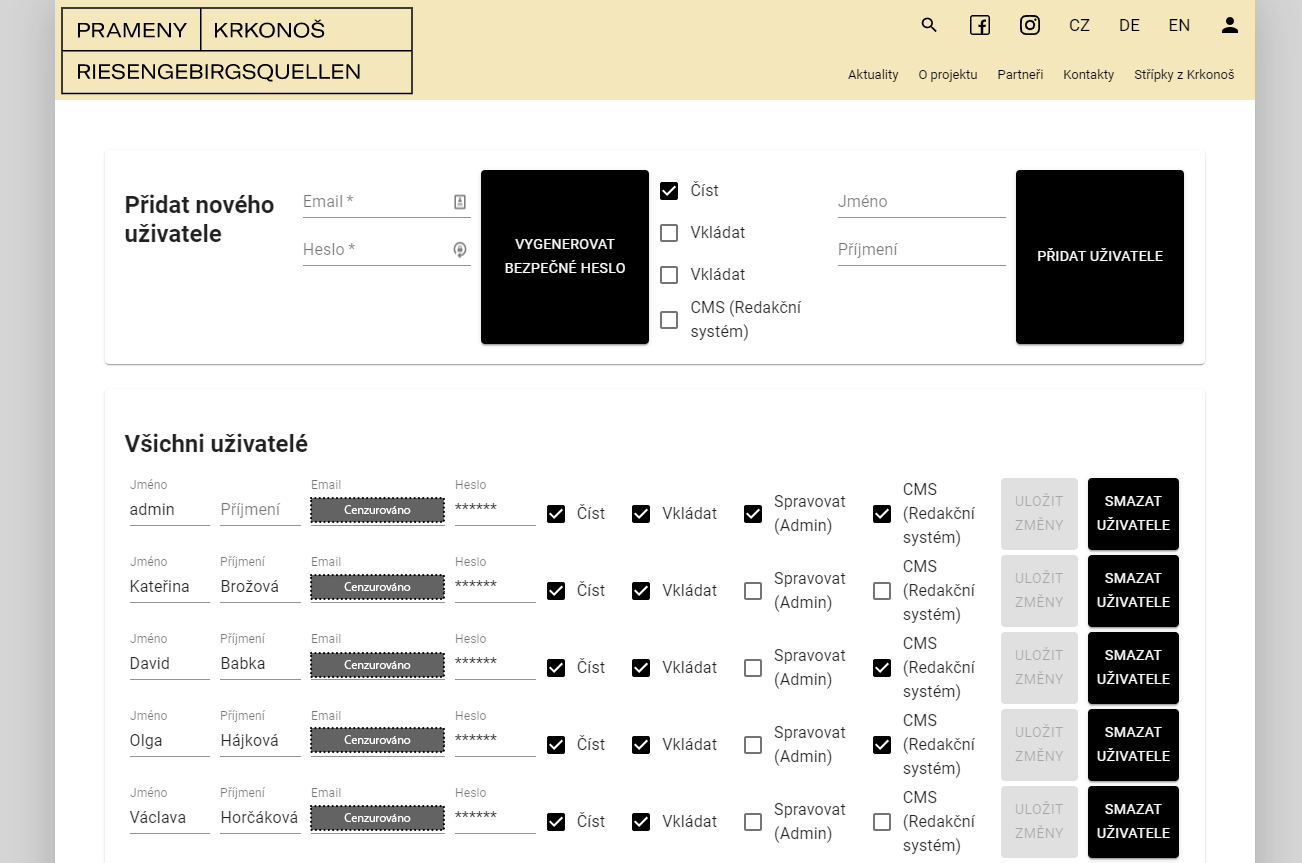
\includegraphics[width=6cm]{img/adminScene.png}
\end{wrapfigure} 
Administrační rozhranní je přístupné pouze s oprávněním \uv{execute}.
Zde může administrátor nebo správce uživatelů konfigurovat vytvořené účty nebo
účty přidávat.

\subsubsection{CMS}
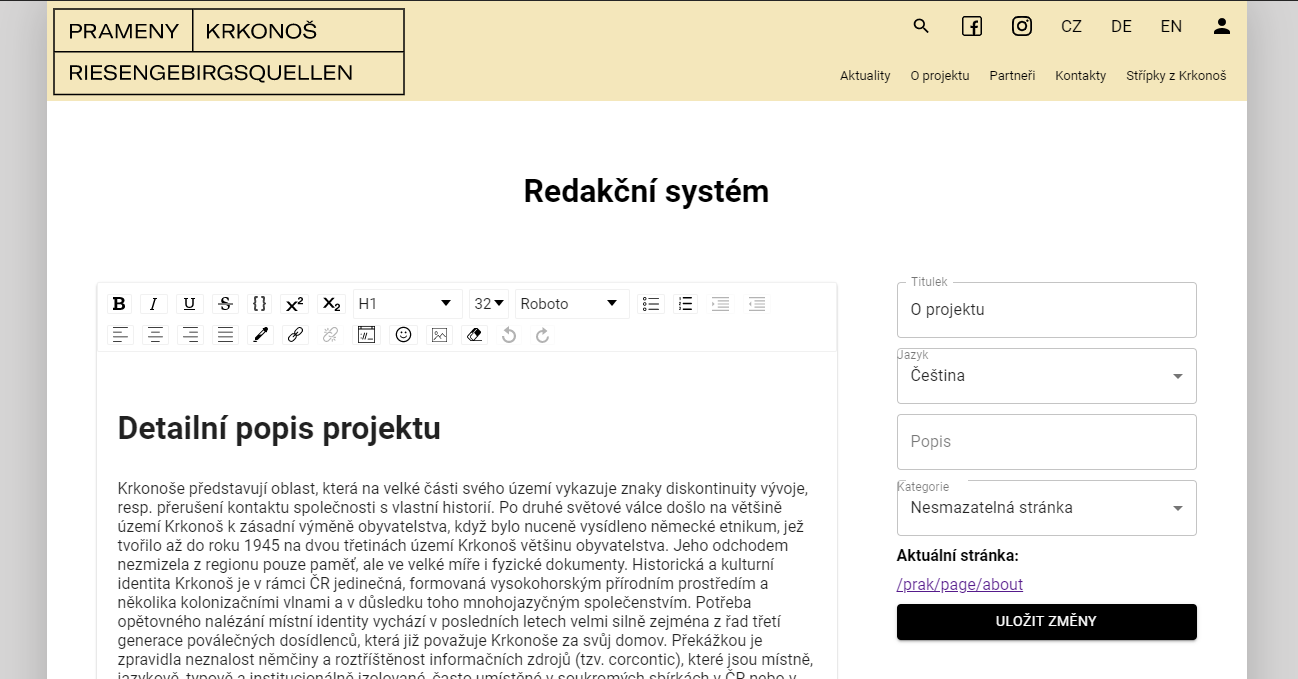
\includegraphics[width=.5\textwidth]{img/cmsScene.png}

\subsubsection{Domovská stránka}
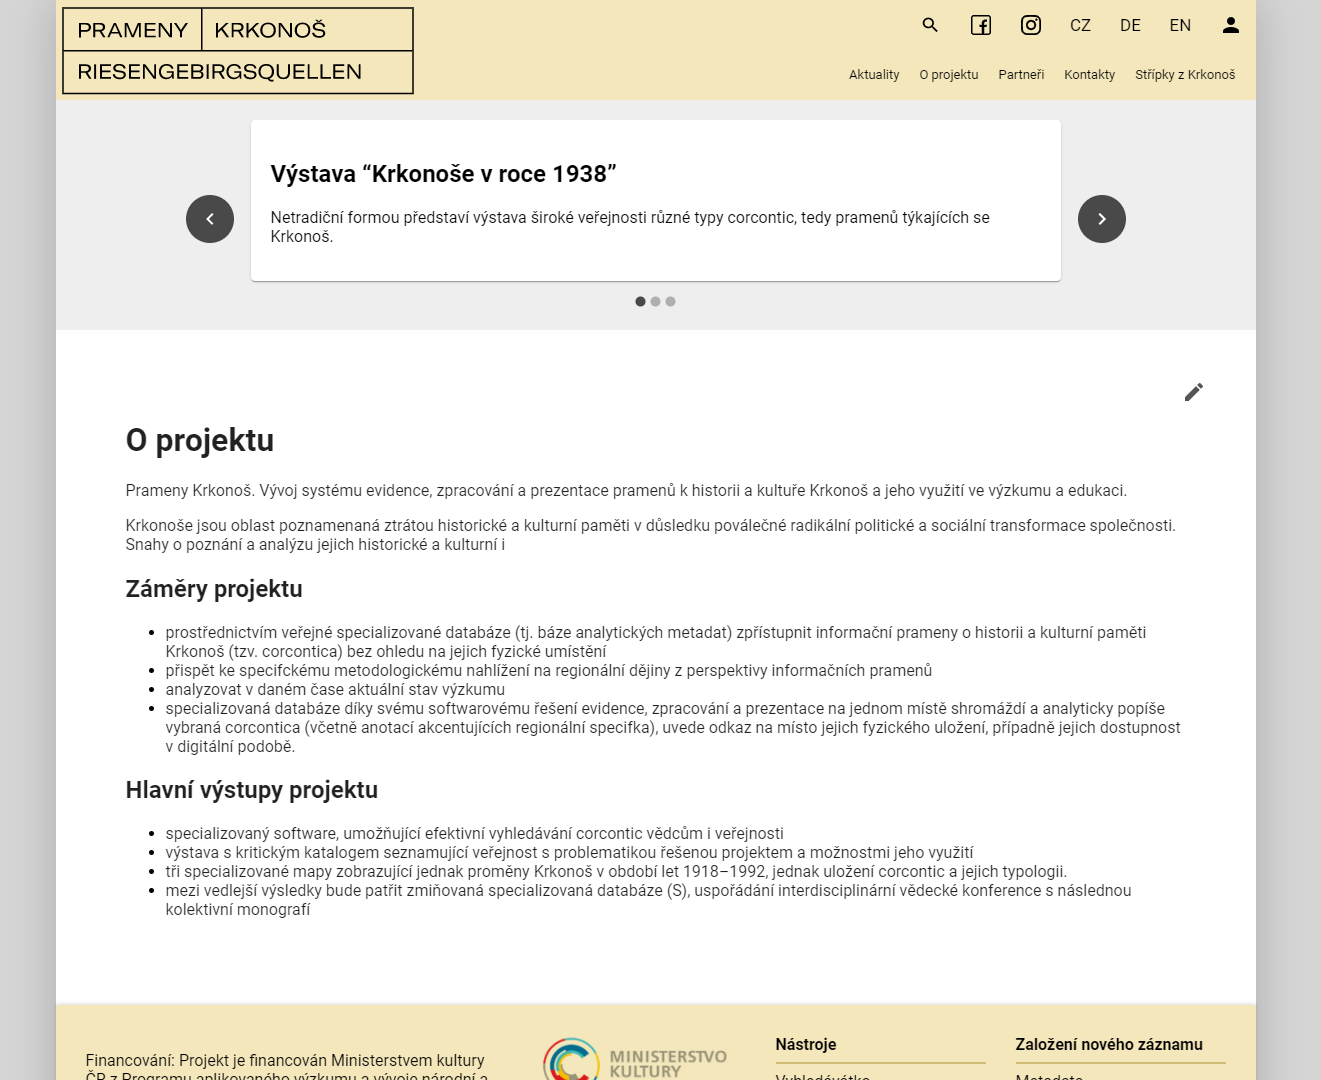
\includegraphics[width=.5\textwidth]{img/homeScene.png}

\subsubsection{Zobrazeni stránky}

\includegraphics[width=.5\textwidth]{img/pageScene.png}

\subsubsection{Přihlašování}
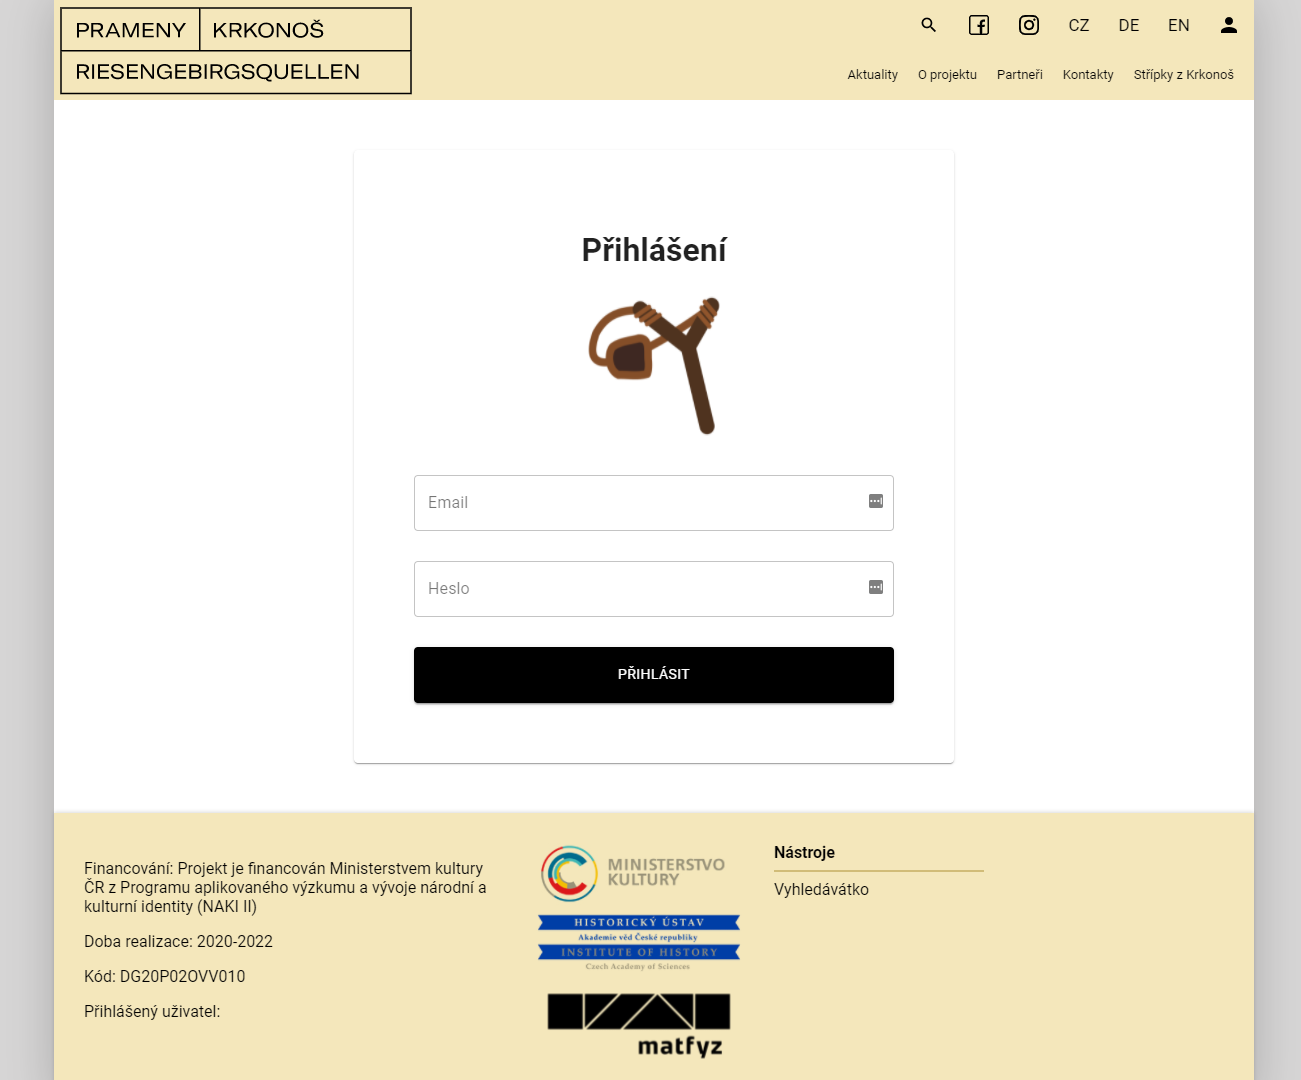
\includegraphics[width=.5\textwidth]{img/loginSceneB.png}
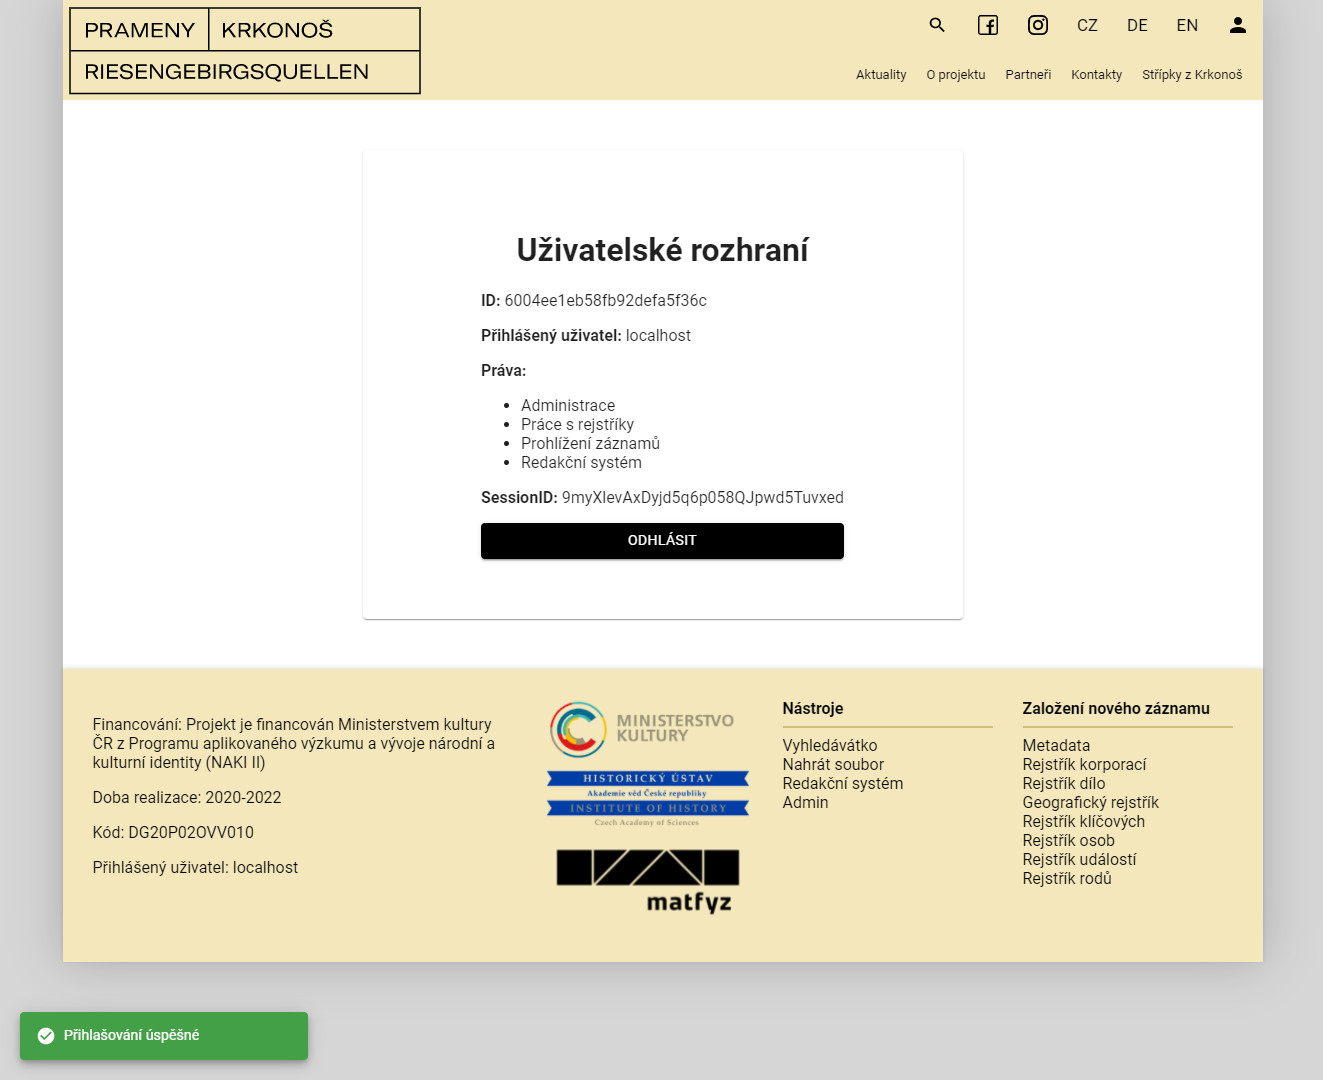
\includegraphics[width=.5\textwidth]{img/loginSceneA.png}

\subsubsection{Kontaktní formulář}
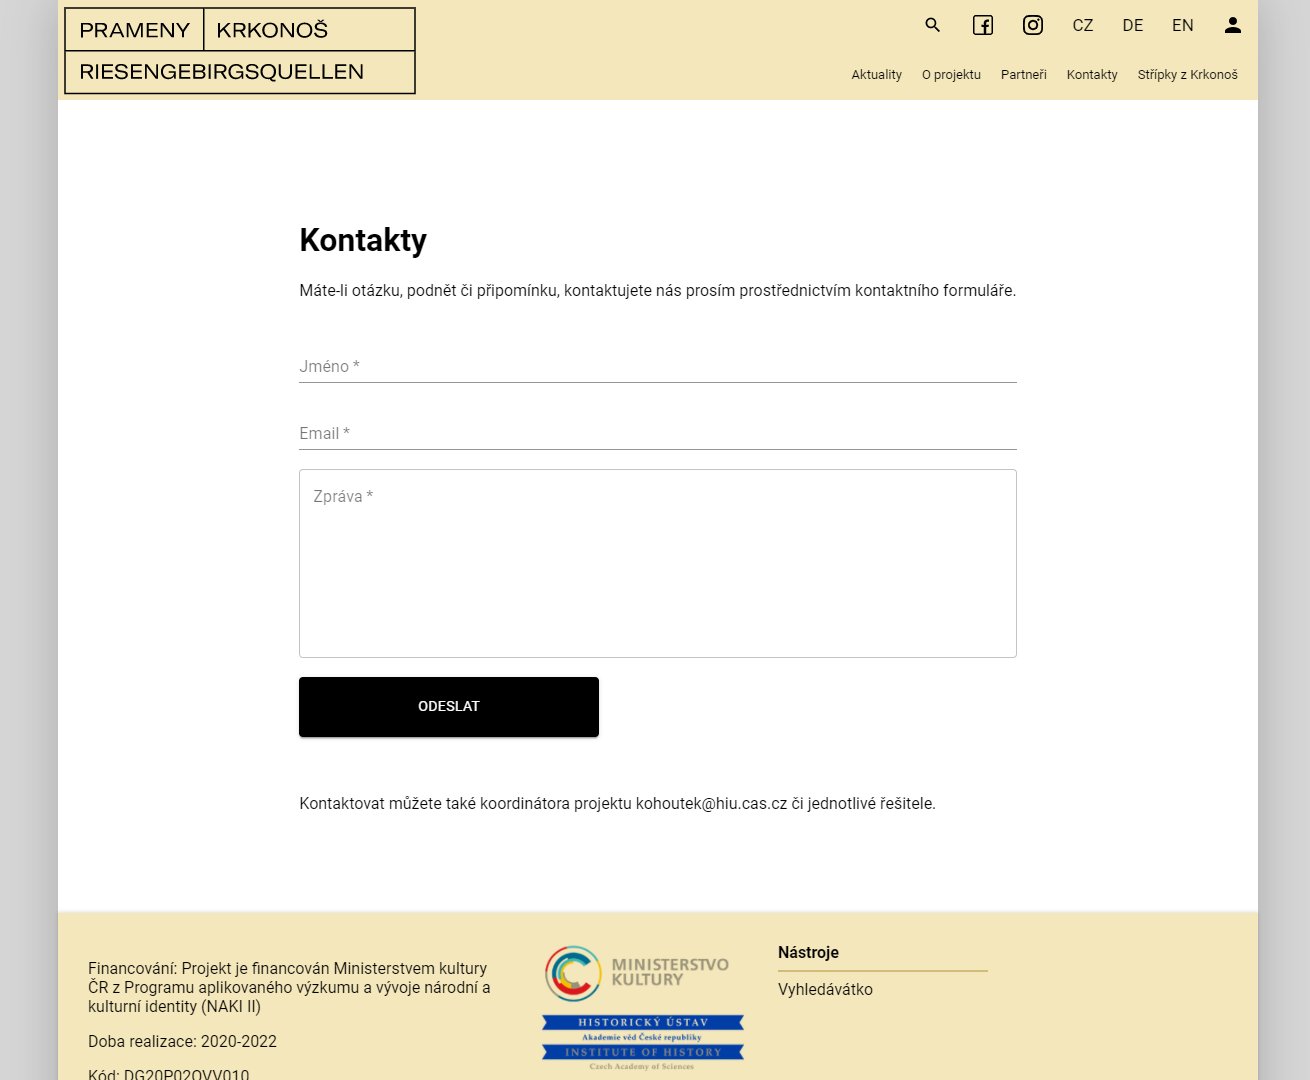
\includegraphics[width=.5\textwidth]{img/contactScene.png}

\subsubsection{Vyhledávátko}
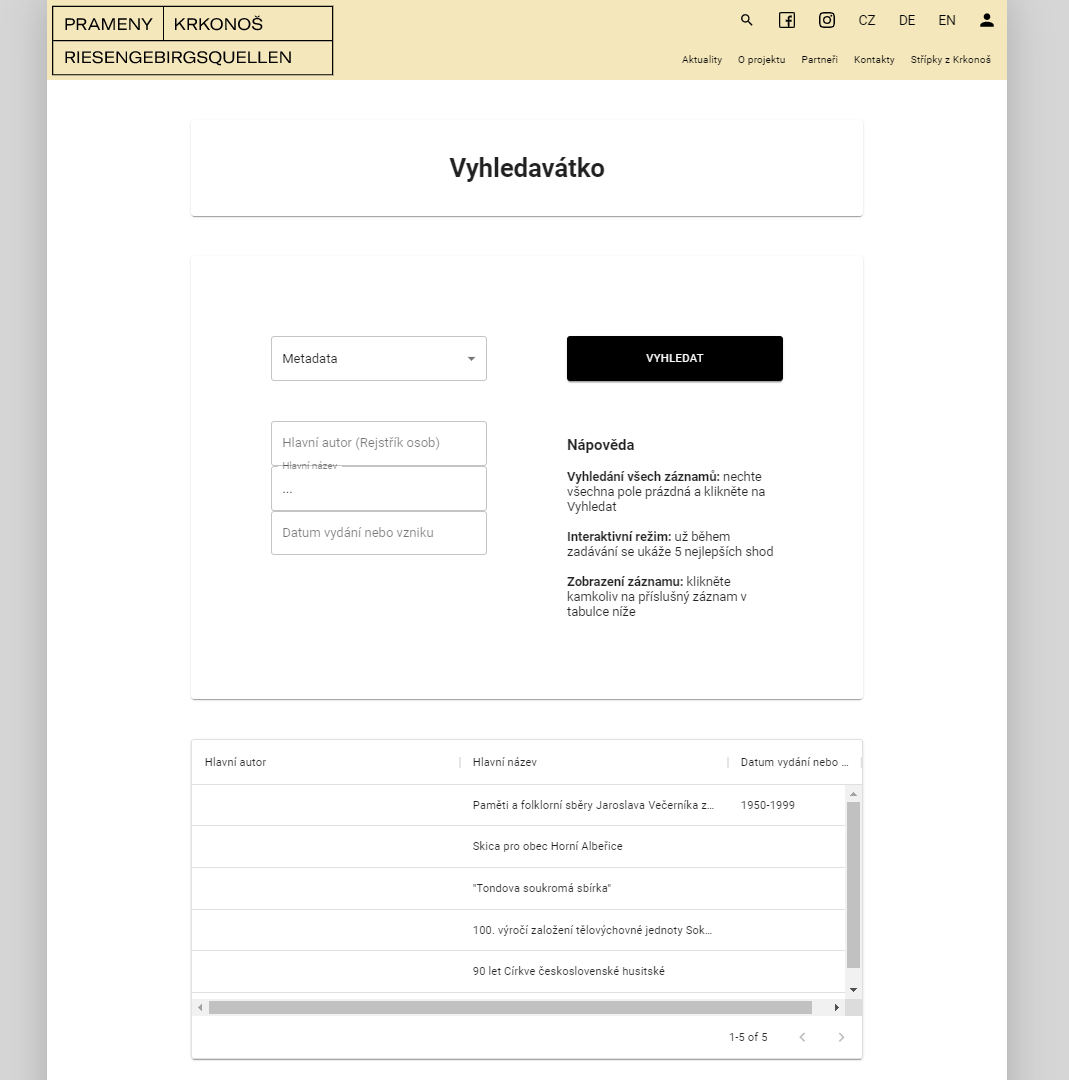
\includegraphics[width=.5\textwidth]{img/searchScene.png}

\subsubsection{Zobrazovávátko}
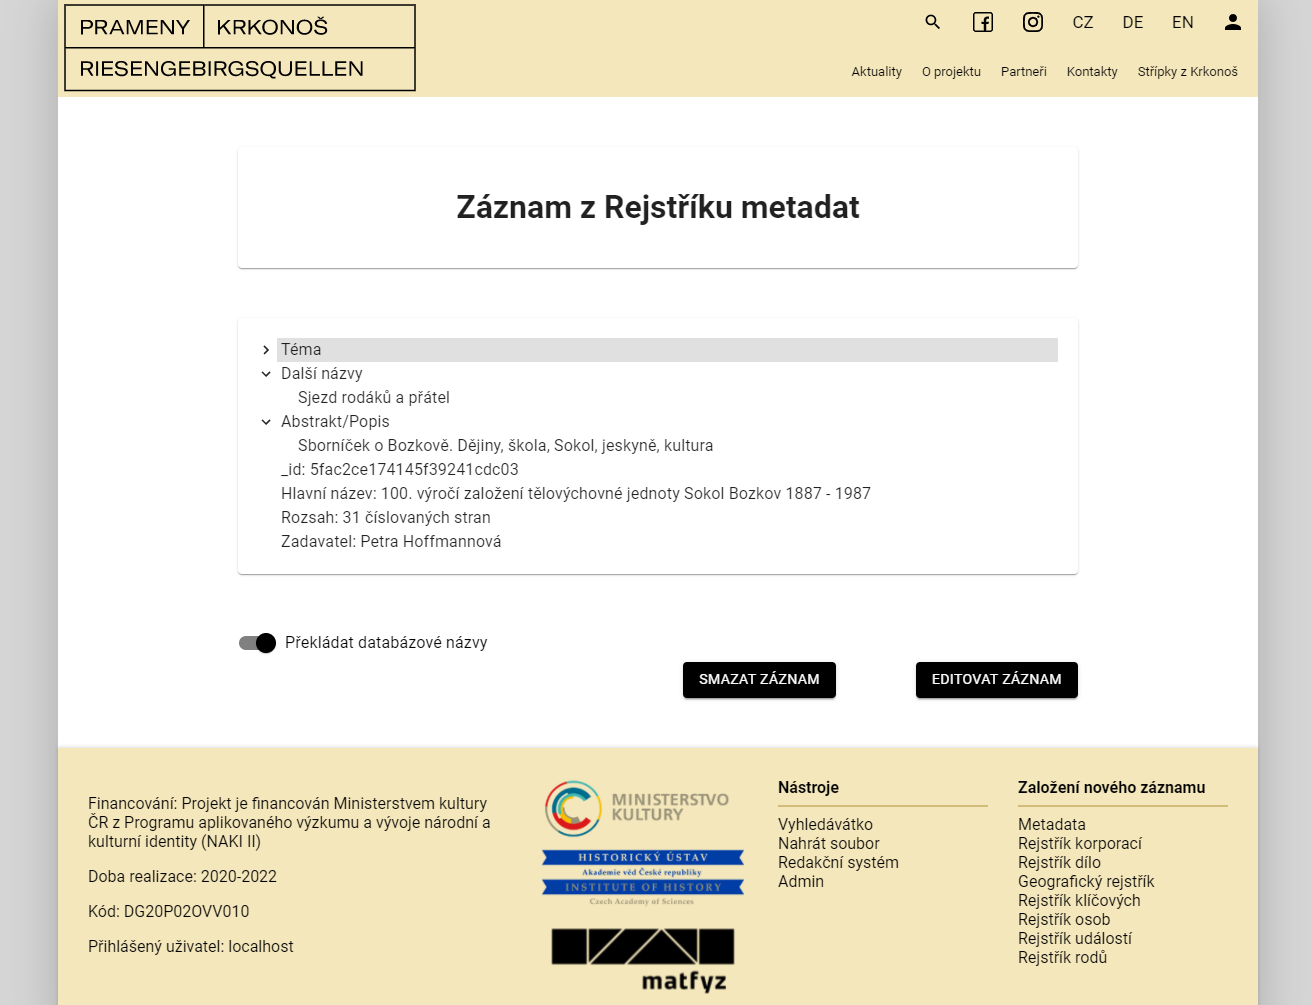
\includegraphics[width=.5\textwidth]{img/showScene.png}

\subsubsection{Upravovátko}
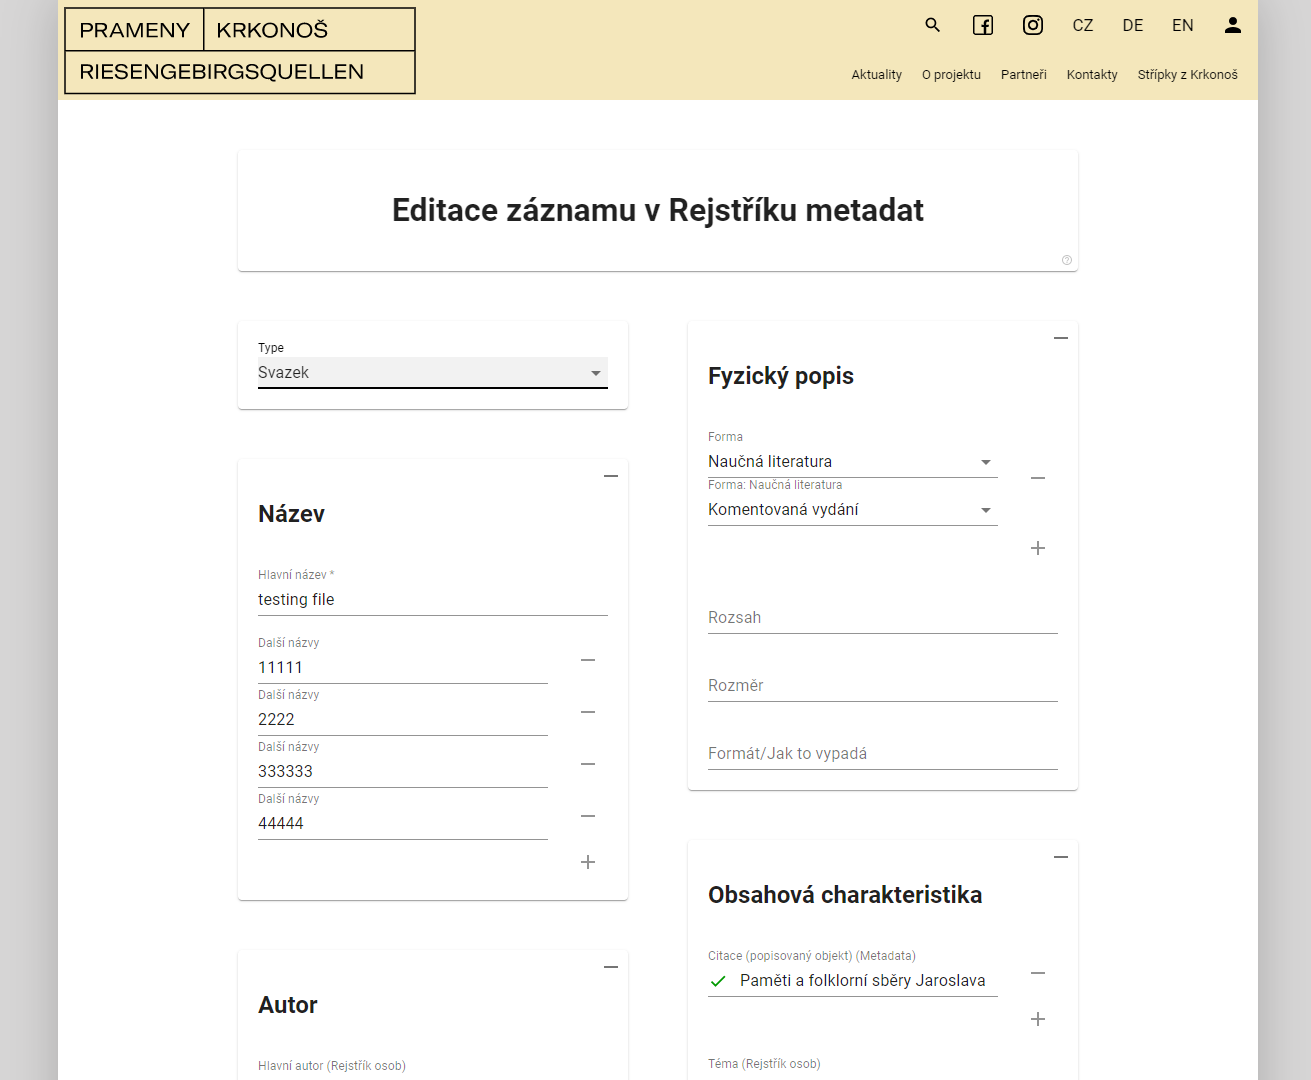
\includegraphics[width=.5\textwidth]{img/editScene.png}

\subsection{Komponenty}
\subsubsection{ComboBox}
\subsubsection{Zápatí}
\subsubsection{Navigační menu}
\subsubsection{Textové pole s validací}
\subsubsection{Pole pro nahrávání souborů}
\subsubsection{Indexy}

\subsection{Moduly}
\subsubsection{Hologram}

\section{Lokalizace}
